\chapter{Introduction}

\section{The Need For Data In Neural Networks}
Deep neural network models dominate as the state-of-the-art machine learning (ML) models that have the best performance across many different image \cite{StableDiffusion1} \cite{YOLOv1} \cite{EfficientNet}, text \cite{BERT}, and video processing tasks applied to multiple disciplines and fields of study. From text generation with large language models (LLMs) such as GPT-3 \cite{GPT3}, object tracking used by the space sector to analyze the sun \cite{Godwill1} and other galactic bodies, object detection used by self-driving cars \cite{SelfDriving1}, to the rise of mobile apps for synthetic audio and image generation that has caught the attention of regular everyday people. Although there are different architectures and different ways to train these networks depending on the task being considered, there is a big commonality among all machine learning (ML) models which is the need to have a lot of data to train these models.

\section{The Difficulty of Getting Data}
Data gathering is one of the most fundamental and important problems in machine learning (ML), as without data there is nothing to train your models with and the quality and quantity of your data makes a big impact on the performance of your given model. The state-of-the-art text generation model GPT-3 \cite{GPT3} was trained on 45TB of text data crawled from the publicly available Internet, Google trained their MLP-Mixer \cite{MLPMixer} and a few other models a 300 million image private subset of the images extracted from their search engine database called JFT-300M, and NVIDIA's StyleGan2 \cite{StyleGAN2} research used the FFHQ dataset which has 70,000 images and the LSUN dataset which has 10 categories with each having from 120,000 to 3,000,000 images.

Although there have been efforts made in different fields to create uniform and useful datasets, data gathering is still one of the main limiting factors preventing researchers of other disciplines from using all the tools and models we have available in deep learning. Data gathering is typically very time consuming, difficult to set-up, and costly in terms of monetary expenses. Big tech companies don't struggle with this problem as much as university researchers and smaller companies do as they have bigger budgets and more staff available for data collection purposes. Even though the research groups as these companies sometimes make their datasets publicly available for others to use \cite{ImageNet} \cite{COCO} \cite{StyleGAN1}, these datasets which usually consist of RGB photographs are not useful to people in other fields of study to solve problems in their respective disciplines. The data needed to solve problems in neuroscience, geology, medicine, and other disciplines will often require advanced equipment, domain experts, and be stored in a different digital format than regular camera photographs.

\section{Working Around Data Limitations With Few-Shot Learning}
The challenges of data gathering and the eagerness of researchers to use neural networks has steadily given rise to a field called ``Few-Shot Learning'' over the years. The idea behind few-shot learning is to train deep neural network models with a ``few'' labeled data samples but still achieve good performance for the given problem. This way you can leverage as much power from these deep neural networks that you can with as little data as possible, making deep neural networks more accessible. Proposed few-shot learning approaches typically focus on taking one component of the traditional deep neural network training pipeline and adapting it to perform better with few training samples. There are 3 main types of approaches, and although I present these approaches as separate fields in the area of ``few-shot learning'' it is not uncommon to have one approach from each field as part of your final model.

\begin{enumerate}
    \item \textbf{Transfer Learning} - Approaches where you take pre-trained models trained on large datasets for a similar problem to yours and then ``transfer'' some of the learned knowledge to your limited data problem.
    \item \textbf{Data Augmentation} - Approaches that propose ways to generate more data samples from your existing ones to increase your dataset size.
    \item \textbf{Meta Learning} - Approaches where your network ``learns to learn'' or extracts some useful knowledge on how to train your network for your problem by training other networks on subsets of other similar data and similar problems in what is called ``episodic training''.
\end{enumerate}

\subsection{Transfer Learning}
In transfer learning the goal is to take models that are already trained and then ``transfer'' as much useful knowledge as possible to your specific problem. This is done by simply loading a trained network, freezing some of the layers so they do not get updated while training anymore, removing the last layer which is usually problem dependent, and adding a last layer that fits your specific problem. 

However, this only works well when the network is pre-trained on data that is similar to yours. The bigger the gap between the domains and problems used for the pre-trained network and your own, the worst the performance will be with transfer learning. Because of this big problem, the cases where you can actually use transfer learning and get good results are few unless you are working with RGB images for the common tasks of object classification or detection. If you are using a different type of input data for a different task, the odds that you will find a pre-trained model with similar data to yours becomes much lower.

\subsection{Data Augmentation}
In data augmentation the goal is to take your existing limited data and generate ``new'' samples from them to increase the size of your dataset. If you have image data, one of the simplest and most popular approaches is to perform simple image processing operations like rotation, cropping, re-sizing, mirroring, and more. However, this requires careful thinking as not all operations will produce good augmentations. For example, for the MNIST \cite{MNIST} hand-written digit dataset it does not make sense to flip or mirror images as the new images will not represent the same digit as the original (a flipped 6 can become a 9). This is one of the disadvantages of data augmentation, the augmentation must still represent the same label as the original data so if your data is not based on images or is complex it may be difficult to come up with rules for data augmentation.

\subsection{Meta Learning}
In meta-learning the goal is to extract useful information that can be used to train your model by training other models and learning how and what those models learned (metadata). For example, let's take the random initialization of networks. Although you can use a uniform or normal distribution, MAML \cite{MAML} proposes learning an initialization that leads to maximal performance on a new problem with a few training steps and a small amount of data. This is done by feeding entire ``problems'' as input data and optimizing the model to produce good results with as few training steps as possible. Therefore you train this model on other problems, and then you feed your specific problem to it so you can also produce good results with few training steps. The drawback of this approach is that it can be computationally expensive to train ``entire problems'' multiple times while optimizing this architecture, the problem of vanishing/exploding gradients is still present in this network, and selecting which extra problems and datasets to use can be a problem as well.

Another popular meta-learning approach is called metric learning. The idea is pretty simple, you might only have a few pictures of zebras and a few pictures of dogs so to classify a new picture you can just compare it to a few of each and find which is the most similar. Thus the main principle is to train models that can compute similarities through metrics. Siamese Networks \cite{Siamese1} are one of the earliest few-shot learning methods proposed to tackle the limited data problem and this approach focuses on metric learning. Siamese Networks take three inputs, a sample from your dataset called an anchor, a sample similar to your anchor called the positive sample, and a sample different to your anchor called a negative sample. Then the network is trained to produce embeddings (1D vectors) such that similar samples are close in that metric space and different samples are further apart, allowing you to use Euclidean distance to find similar samples. This idea was further improved in Prototypical Networks \cite{PrototypicalNetworks}, where the idea is now to find ``prototypes'' or samples that represent a general class of similar objects instead of having the triplets. For example, you may find one of your pictures is a good representation of ``mammals'' and can make it easier to identify new mammals in the future. In Relation Networks \cite{RelationNet} this metric learning idea is generalized even more. Specifically, the authors propose an end-to-end two-part network that is trained to learn a custom distance metric used to compare pairs of images called a ``relation score'' instead of always using Euclidean distance. Then when a new image needs to be classified, we can compare it against our few labeled samples and find the most similar one or the one with the highest ``relation score''. As the distance metric used for comparison is custom learned, the model performs better than if you used general distance metrics like Euclidean distance or Cosine similarity like in \cite{PrototypicalNetworks} or \cite{Siamese1}. These type of architectures, however, are typically designed for image classification problems and cannot be used as-is for more complex tasks like image segmentation or object detection or for other types of input data that are not regular camera RGB images.

\section{Few-Shot Learning By Integrating Physics Into Neural Networks}
\label{Few-Shot Introduction}
One of the reasons why humans might be able learn new things with few examples and do few-shot learning is because we have a lot of previous knowledge that we leverage in our learning process and we never truly start from scratch as deep neural networks do. My research focus is then on how we can integrate our knowledge of physics to improve neural network performance and have models more ``easily learn'' with few examples, mimicking humans. Physics is a widely studied area of science that has been researched for hundreds of years for which we not only have a lot of mathematical equations but also a lot of expertise and knowledge in the field. As many problems across different disciplines are based on real-world data they must follow the ``laws of physics'' and so we can leverage our knowledge of physics to help improve performance on limited datasets that deal with real world data. 

% The aim is to make it easier for researchers of other disciplines to collaborate in interdisciplinary projects that use deep neural networks by requiring less data gathering and allowing them to use current state-of-the-art models to solve problems in their fields.

There exists an area of study called Physics-Informed Neural Networks (PINNs) \cite{PINNS} where the aim is to integrate physics that can be described as systems of partial differential equations (PDEs) directly into the loss function of a network. Unless you are working with simulation data, it will be close to impossible to collect all the variables and data needed to describe how your specific problem behaves exactly at all times. There is just too much data at too many different scales, from quantum effects all the way to space-time gravitational influences. Due to this, scales and times are often discretized when working with these PDEs like when using the Finite Element Method (FEM) to compute solutions for these PDEs. PINNs allow you to model some of these intrinsic variables of your data and use them along with the laws of physics (PDEs) that describe how they interact to increase your model performance. I will be extending this area by creating new network models and loss functions that will allow us to integrate PINNS and other neural network models to solve problems from two disciplines that have limited datasets.

\section{Specific Problems From Other Disciplines That Have Limited Datasets}
As my research focus is on applying physics to neural networks to improve model performance on problems with limited datasets I selected problems from two disciplines that had limited data available and whose data must follow the ``laws of physics'' in some way. Those problems were ``Fluid Flow Velocity Prediction'' from mechanical engineering and ``Glacial Ice Segmentation'' from geology.

\subsection{Fluid Flow Velocity Prediction}
Understanding how fluids flow is very important for the study and development of airplanes, cars, boats, rockets, and much more. One of the widely researched approaches used to study fluid flow is setting up Computational Fluid Dynamic (CFD) simulations using software developed specifically for that purpose like Ansys Fluent\cite{ANSYS}. It is unfeasible to model every particle of every fluid we are interested in modeling at every scale and every point in space due to computational and time limitations, so it is necessary to define a discretized mesh of finite elements of specific size as shown in Figure \ref{fig:cfd_mesh} below.

\begin{figure}[H] \centering
    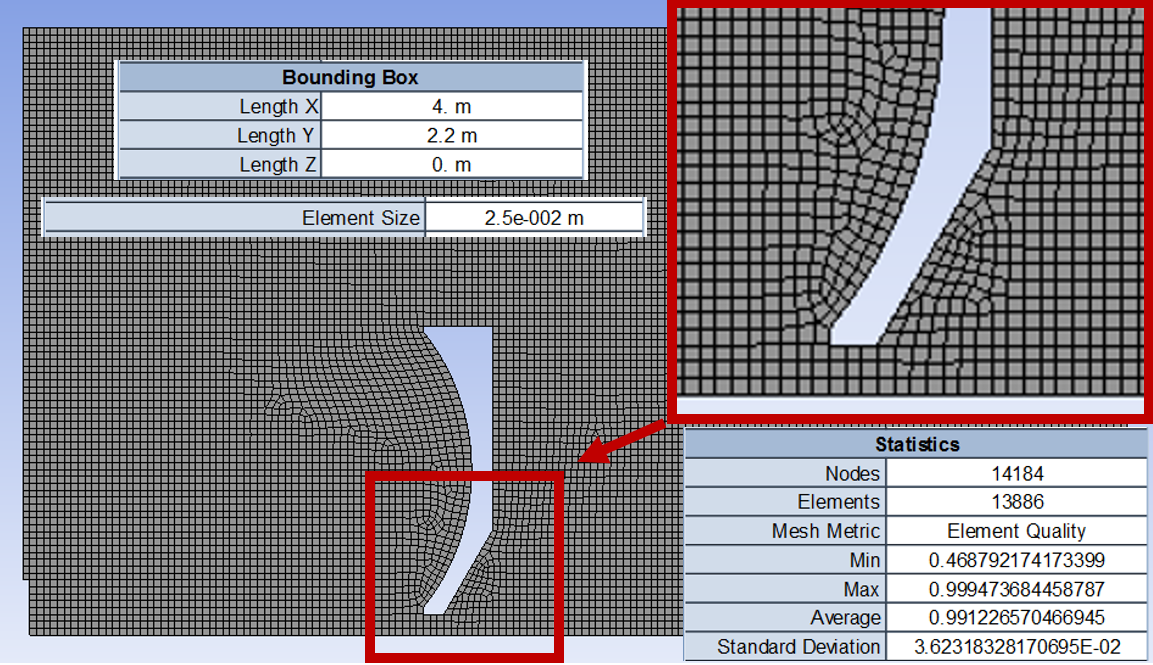
\includegraphics[width=\linewidth]{figures/cfd_mesh.png}
    \caption{Example of a discretized mesh of finite elements used for a CFD fluid flow simulation.}
    \label{fig:cfd_mesh}
\end{figure}

After deciding the scale which we are interested in modeling and studying, the next step is to define the relevant geometry, fluids, and boundary conditions for the simulation as show in Figures \ref{fig:cfd_geometry} and \ref{fig:cfd_boundary_conditions} below. Lastly, a solver is selected and the simulation is run for a specific period of time.

\begin{figure}[H] \centering
    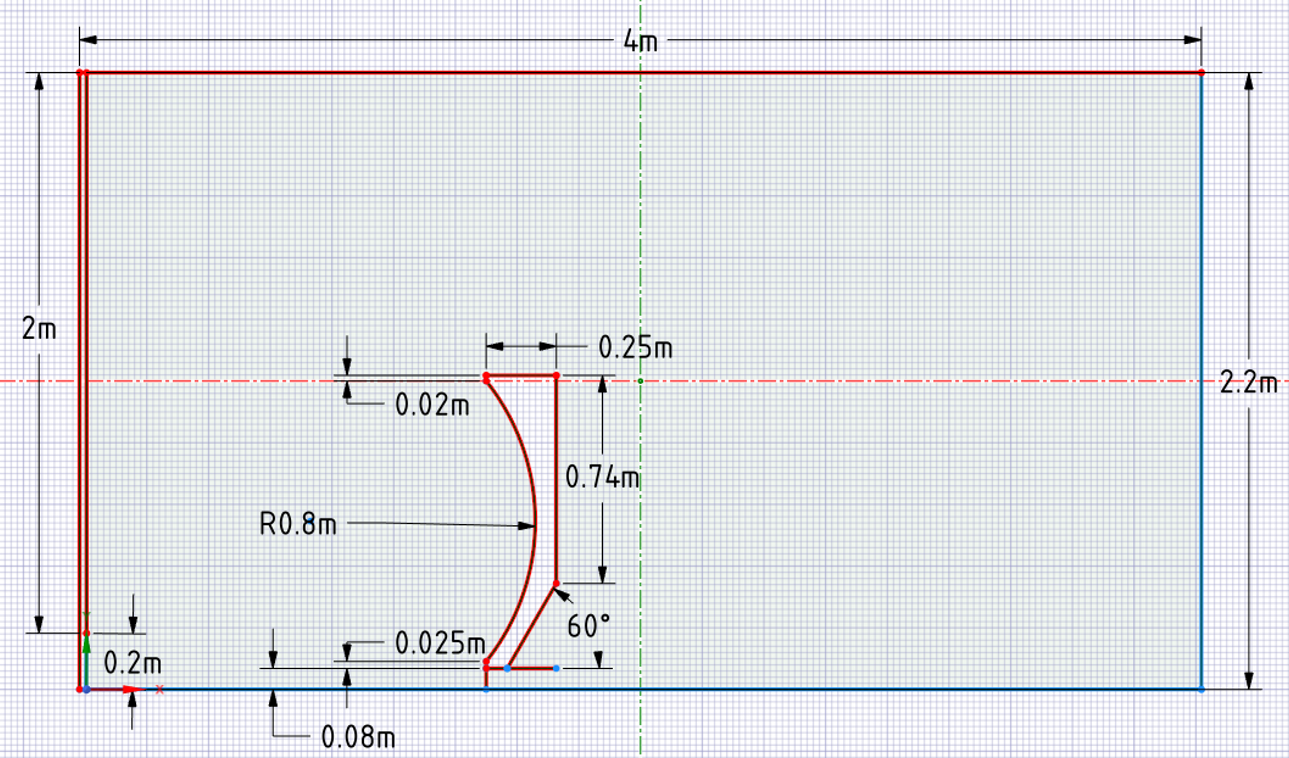
\includegraphics[width=\linewidth]{figures/cfd_geometry.png}
    \caption{Example of geometry used for a CFD fluid flow simulation. This modeled geometry is for a proposed water-braking mechanism for a pusher sled system used in the Holloman Air Force Base for experiments.}
    \label{fig:cfd_geometry}
\end{figure}

\begin{figure}[H] \centering
    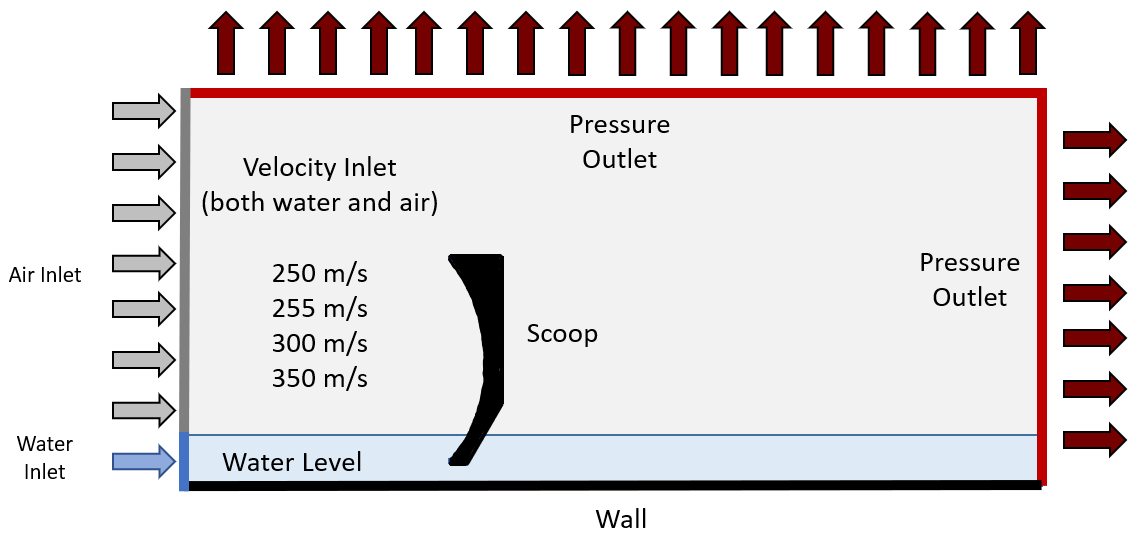
\includegraphics[width=\linewidth]{figures/cfd_boundary_conditions.png}
    \caption{Example of boundary conditions used for a CFD fluid flow simulation. These boundary conditions model how the geometry (water-breaking scoop) will interact with the water as the pusher sled mechanism pushes the scoop at specific initial velocities.}
    \label{fig:cfd_boundary_conditions}
\end{figure}

One drawback of CFD simulations is that high-fidelity simulations can be very computationally expensive as having smaller finite elements, bigger meshes, bigger geometries, and bigger simulation environments increases the computations needed for the solvers to simulate each given time-step of the simulation. Although fluid flow datasets are available for some problems in fluid dynamics, many researchers are interested in fluid flows for specific problems with different geometries and boundary conditions than those in the available datasets. As fluid flows are a widely studied area in mechanical engineering in the field of fluid dynamics, we know that the Navier-Stokes equations can be used to describe some of these flows and that these equations are partial differential equations (PDEs) allowing us to leverage Physics-Informed Neural Networks \cite{PINNS} to tackle this limited data problem.

\subsection{Glacial Ice Segmentation}
Glaciers are a very important source of water for people and wildlife of many different regions of the world, as not only do they provide a source of drinking water but also water for watering crops and generating hydroelectric power \cite{GlacierImportance}. As these regions rely heavily on glacial melt as a water source, it is important to monitor and keep track of changes that happen to these glaciers over time. 

There exists multiple satellites such as NASA's Landsat-7, Landsat-8, and Sentinel-2 that have captured hyperspectral images of these glaciers over a long period of time, allowing glaciologists to take these images and use their expertise to determine what areas of the images are clean ice, debris covered ice (ice mixed with rocks), and regular rocks in a process called glacier mapping. This is one of the ways that these scientists monitor the glaciers over time, and in the area of computer vision is called image segmentation. An example of this is given in Figure \ref{fig:glacier_mapping} below.

\begin{figure}[H] \centering
    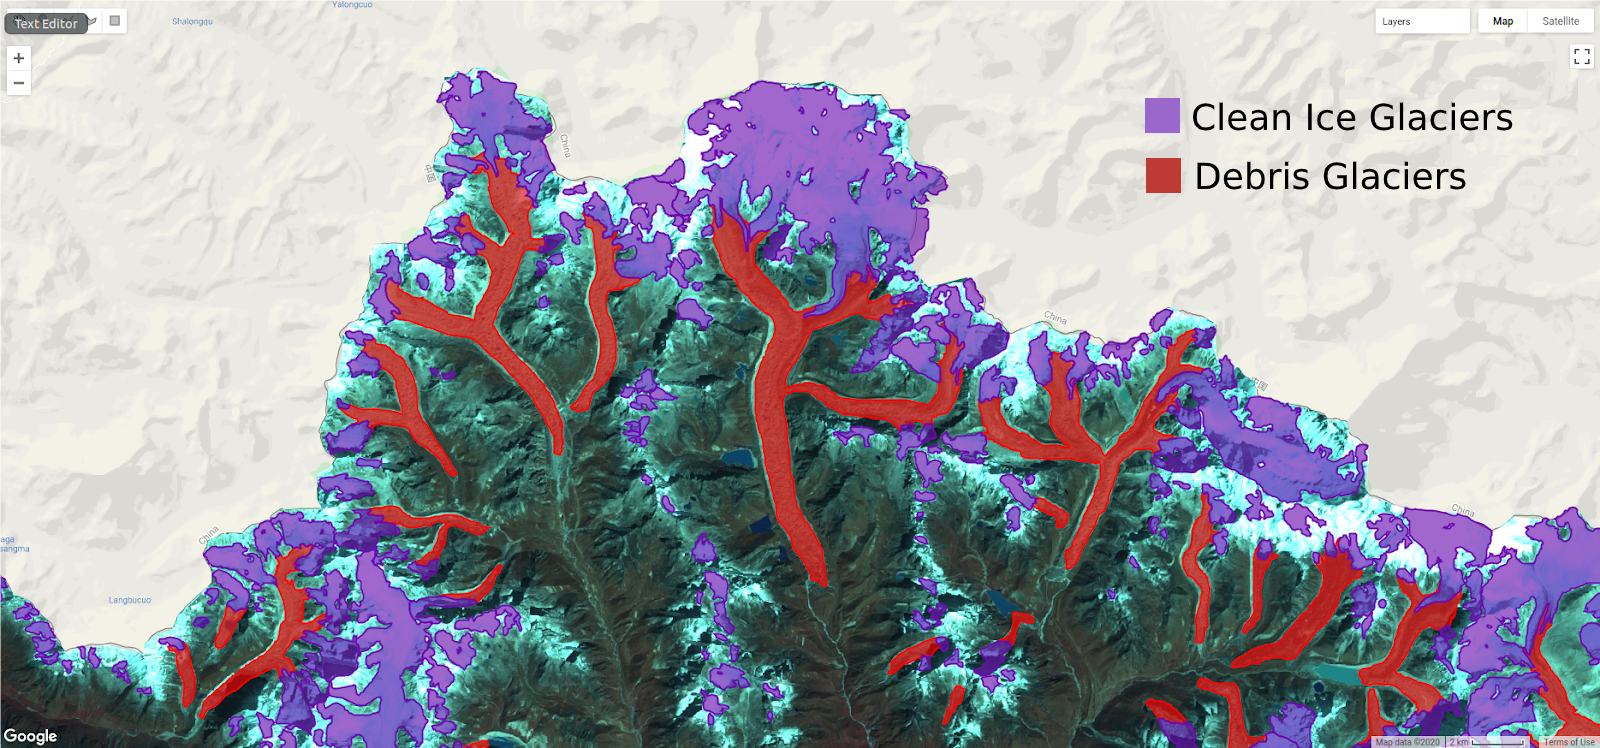
\includegraphics[width=\linewidth]{figures/glacier_mapping.png}
    \caption{Example of glacier mapping or segmentation of a satellite image into clean ice and debris covered ice glaciers.}
    \label{fig:glacier_mapping}
\end{figure}

However, manually labelling hyperspectral satellite images into clean ice and debris covered ice glaciers is a very time consuming task. This is due to two main reasons:

\begin{itemize}
    \item Satellite images have more channels than the regular 3 (RGB) in digital cameras, so they are hyperspectral images and require the usage of specialized tools (like QGIS) and knowledge about what channels capture which bands of the electromagnetic spectrum to properly visualize and analyze.
    \item High resolution images are difficult to segment as there are too many individual pixels, and although glaciologists use tools such as QGIS to label the images using geometric shapes instead of pixel by pixel to speed up the process it is still time consuming and difficult to label the borders/boundaries between the clean ice and debris covered ice specifically due to the amount of fine detail and care needed.
\end{itemize}

Labeling a single patch of a glacier using Sentinel-2 satellite imagery can take an expert 1 to 4 weeks depending on the complexity of the image, and the Hindu-Kush Himalayas (HKH) glaciers are made up of at least 256 of such patches.

A labeled dataset exists for the glaciers in Hindu-Kush Himalayas (HKH) region created by the International Centre for Integrated Mountain Development (ICIMOD) for images taken with NASA's Landsat-7 satellite. These images contain 7 channels including RGB, Near-Infrared, and Digital Elevation Map data. 

There also exists a dataset of glacier ice velocities created by the National Snow and Ice Data Center containing the surface velocities of major glacier-covered regions in the world including the Hindu-Kush Himalayas (HKH) spanning from 1985 to 2018 and compiled from multiple of NASA's Landsat satellites called the ``MEaSUREs ITS\_LIVE Regional Glacier and Ice Sheet Surface Velocities'' dataset. As glacial ice velocity prediction is a specialized form of fluid velocity prediction where the fluid being analyzed is ice from the glaciers, we can use the Navier-Stokes equations once again to leverage Physics-Informed Neural Networks \cite{PINNS} to help us tackle this limited data problem.

\section{Thesis Statement}
% Using partial differential equations
% physics-informed data augmentation and loss function design
% a little more specific towards the work I completed
Incorporating physics in neural network models through modification of data and loss functions will allow for better performance and faster convergence for the problems of fluid flow velocity prediction and glacial ice segmentation.

% \begin{enumerate}
%     \item \textbf{Problem Determination} - Determining what exactly is the problem we want to solve and how to set it up as a data problem that can be solved using machine learning (ML) models. 
%     \item \textbf{Data Gathering} - Collecting or finding a source of data for the problem we want to solve.
%     \item \textbf{Baseline Preparation} - Determining and implementing baselines to determine if our approach is actually doing better than other approaches and what metrics should be used for comparison and evaluation.
%     \item \textbf{Neural Network Architecting} - Determining what neural network architecture will be used and what other techniques from few-shot learning need to be applied to solve this problem.
%     \item \textbf{Experimentation} - Training and evaluating different neural networks to find the best performing model.
% \end{enumerate}

% I defined the fluid flow velocity prediction problem as the ML task called ``Next-Frame Prediction'' and the glacial ice segmentation problem as the ML task called ``Image Segmentation''. In each chapter I will be discussing approaches I used or propose to use to solve these tasks in detail along with the specific data gathered, baseline preparations, network architectures, and experimental results. The bulk of my research contributions will be in the architecting of the neural networks as that is where I will be integrating the physics into the models. I will specifically do so by creating new loss functions, new architectures based on previously proposed literature models, and by augmenting the limited data I gathered with ``Physics-Aware'' input channels.

\section{Expected Contributions}
The proposed contributions of this research are as follows:

% **SPLIT FURTHER... GENERALIZE NO NEED FOR SPECIFICS.. VARIABLES MISSING (TEMPERATURE, ETC) BUT WE KNOW VERY LITTLE IN GLACIER MAPPING VS FLUID FLOW. INVESTIGATE NETWORKS THAT EXPLOIT SEQUENCE...ETC..WAYS TO AUGMENT DATA...**

% A lot of variables => Be specific
% Typically, all scales/times discretized like in the fininte element method
% My idea is to exploit the fact that the laws of physics have to be followed / the real world follows the laws of physics / there are some things that the neural network does not need to learn
% 

\begin{enumerate}
    \item \textbf{A physics-informed neural network model for the task of fluid flow velocity prediction} - We will develop a model that uses Physics-Informed Neural Networks (PINNs) \cite{PINNS} for the task of fluid flow velocity prediction and investigate ways to combine PINNs with networks built for sequential data (such as \cite{LSTM}) to take advantage of how fluid flows over time sequentially allowing for improvements on network convergence speed.

    \item \textbf{A neural network model with physics-informed data augmentation for the task of glacier mapping} - As there already exists a network for glacier mapping by image segmentation \cite{Bibek2023}, we will investigate ways to augment the current available labeled data for glacier mapping based on physics, improving the performance of the pre-existing segmentation model. 

    \item \textbf{A physics-informed neural network model for the task of glacial ice velocity predictions} - Glacial ice velocity prediction is a subset of the general fluid flow velocity prediction problem, allowing us to use Physics-Informed Neural Networks (PINNs) \cite{PINNS} combined with networks built for sequential data (such as \cite{LSTM} and \cite{Attention1}) to leverage the fact that glacial ice flows over time (sequentially) for the task of glacial ice velocity prediction.

    \item \textbf{A physics-informed neural network model for the task of glacier mapping} - We will develop a new model based on a combination of Physics-Informed Neural Networks (PINNs) \cite{PINNS} and a pre-existing segmentation model \cite{Bibek2023} for the task of glacier mapping by segmenting glacier ice in satellite images. We will investigate ways to combine datasets containing hyperspectral satellite images that have no velocity information and datasets of ice glacier velocities to leverage the knowledge we have about the physics of ice glacier velocity flows and achieve better performance on the segmentation of glacier ice.

    % \item \textbf{A neural network architecture with physics-informed data augmentation for the task of glacier mapping} - There are a lot of variables that affect how glaciers behave in the real world and although we can observe them with satellites and sensors the current datasets for glacier mapping do not always include these variables at every point in time and at every scale. As there already exists a network for glacier mapping by image segmentation \cite{Bibek2023}, we will investigate ways to augment the current available labeled data for glacier mapping based on physics, improving the performance of the pre-existing segmentation model. 
    
    % \item \textbf{A physics-informed neural network architecture for the task of glacial ice velocity predictions} - Glacial ice velocity prediction is a subset of the general fluid flow velocity prediction problem so we know there are a lot of variables affecting it that are not present in the current labeled datasets. We will develop a model that uses Physics-Informed Neural Networks (PINNs) \cite{PINNS} to capture and model some of those intrinsic variables and investigate ways to combine PINNs with networks built for sequential data (such as \cite{LSTM} and \cite{Attention1}) to leverage the fact that glacial ice flows over time (sequentially) for maximum performance on the task of glacial ice velocity prediction.
    % \item \textbf{A physics-informed neural network architecture for the task of glacier mapping} - We will develop a new architecture based on a combination of Physics-Informed Neural Networks (PINNs) \cite{PINNS} and a pre-existing segmentation model \cite{Bibek2023} for the task of glacier mapping by segmenting glacier ice in satellite images. We will investigate ways to combine datasets containing hyperspectral satellite images that have no velocity information and datasets of ice glacier velocities to leverage the knowledge we have about the physics of ice glacier velocity flows and achieve better performance on the segmentation of glacier ice.
    
    
    % \item \textbf{A neural network architecture for time series data that incorporates physics for the task of fluid flow velocity predictions} - We developed Physics-Informed LSTMs \cite{Perez2022}, a novel architecture combining Physics-Informed Networks (PINNs) \cite{PINNS} and Long Short-Term Memory Networks (LSTMs) \cite{LSTM}, and tested them with fluid flow simulation data, demonstrating the viability of using physics to improve performance in terms of training speed and accuracy on neural networks with limited data. We will apply this architecture to glacier velocity data and experiment with different modifications to the architecture to find an optimal architecture for the glacier mapping task.
    % \item \textbf{A neural network architecture for hyperspectral satellite images that incorporates physics for the task of glacier mapping} - We developed Physics-Informed Data Augmented UNet, a model which computes an extra channel from the hyperspectral satellite images based on some assumptions made through observation of glacier physics, and through it demonstrated the viability of using physics to improve performance on the task of glacier segmentation. We will develop a novel architecture that combines Physics-Informed Neural Networks (PINNs) \cite{PINNS} and UNet \cite{UNet} which will be able to be used for that same task.
    % \item \textbf{Tool for faster glacier mapping} - We will develop a semi-automated system for the mapping of glaciers given hyperspectral satellite images. This system will use the models trained for glacier ice segmentation that are augmented with physics proposed in \#2 and produce masks of glacier labels that can then be loaded in QGIS, a tool often used by glaciologists for manual glacier mapping. Glaciologists will then be able to edit and correct these masks, speeding up the manual mapping process as they won't have to start from scratch for every single image they want to label.
\end{enumerate}

% \newpage
% \section{Timeline}
% To view the current graphical timeline more clearly, please see it on Google Docs:
% \url{https://docs.google.com/spreadsheets/d/1QdJVmF3Ofcg3Fgk2A4Auc5od6M4ocpm2C0jPb-eUnIQ/edit?usp=sharing}

% \begin{figure}[hbtp]
%     \makebox[\linewidth]{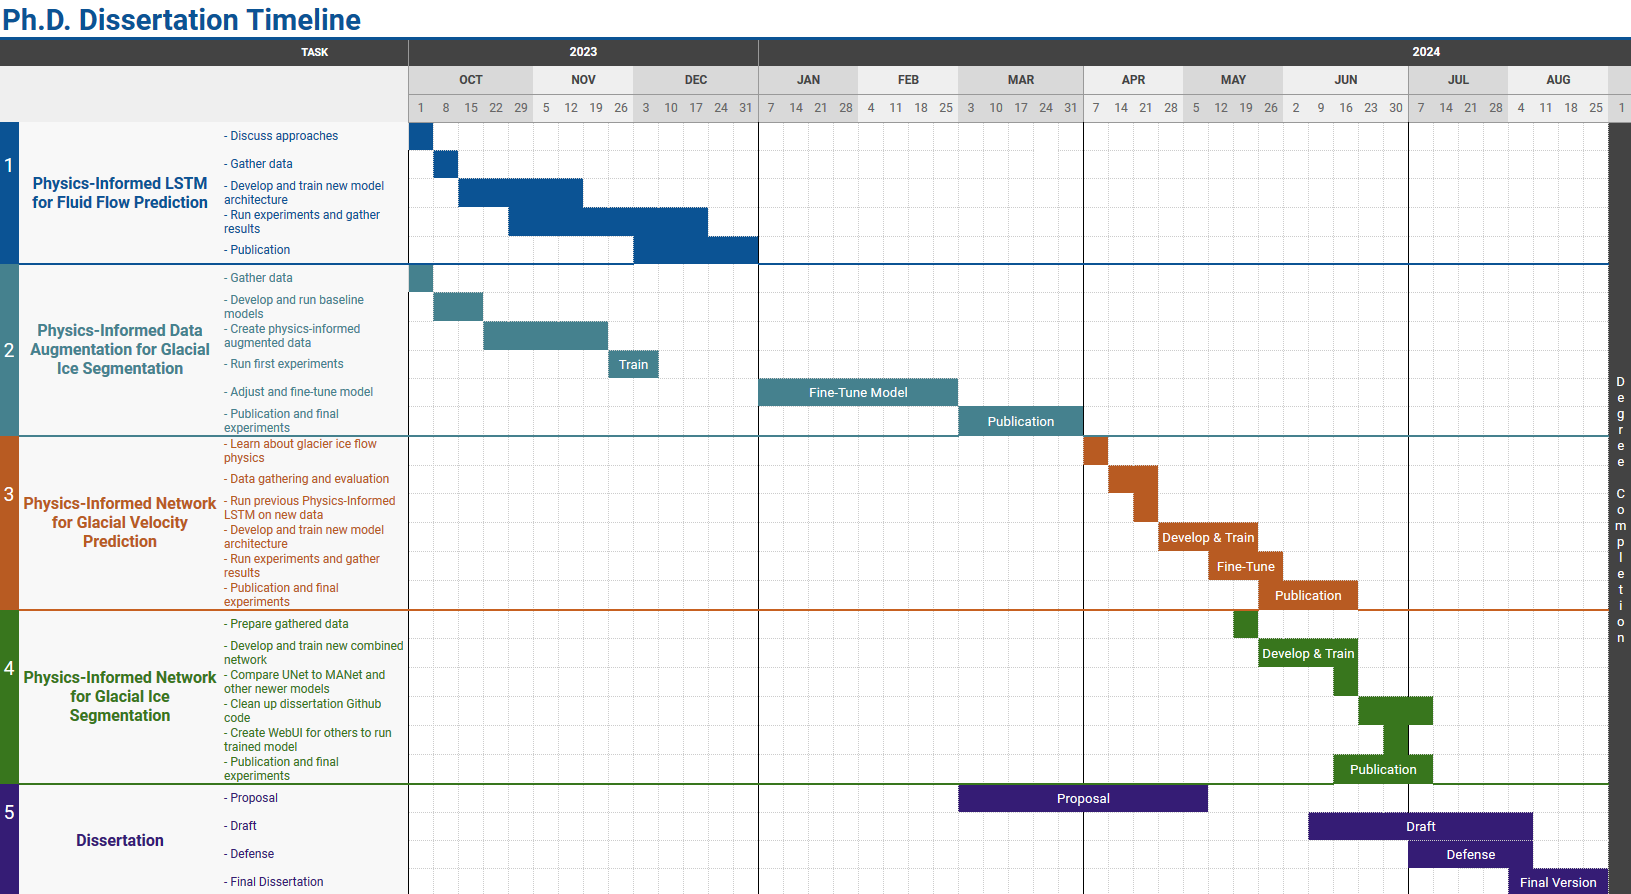
\includegraphics[scale=0.5]{phd_timeline.png}}
%     \caption{Proposed timeline visualized graphically.}
%     \label{fig:timeline}
% \end{figure}

% The table below breaks down the timeline per task, and many tasks will be running concurrently throughout the timeline.
% \begin{table}[ht!]
%     \centering
%     \begin{tabular}{l|c}
%         \toprule
%          Task & Duration \\ 
%          \midrule
%          \textbf{Physics-Informed LSTM for Fluid Flow} & 3 Months \\ \hline
%          - Discuss approaches with Dr. Kumar's students & 1 Week \\
%          - Gather data from Dr. Kumar's students & 1 Week \\
%          - Develop and train new model architecture & 5 Weeks \\
%          - Run experiments and gather results & 8 Weeks \\
%          - Publication & 5 Weeks \\ \hline
%          \textbf{Physics-Informed Data Augmentation for Glacial Ice Segmentation} & 3 Months \\ \hline
%          - Data gathering & 1 Week \\
%          - Baseline models & 2 Weeks \\
%          - Created physics-informed augmented data & 5 Weeks \\
%          - First experiments & 2 Weeks \\
%          - Adjustments to model and data for improved performance & 8 Weeks\\
%          - Publication & 5 Weeks \\ \hline
%          \textbf{Physics-Informed Net for Glacial Velocity} & 3 Months \\ \hline
%          - Learning about glacier ice flow physics & 1 Week \\
%          - Data gathering and evaluation & 1 Week \\
%          - Running previous Physics-Informed LSTM on new data & 1 Week \\
%          - Creating and evaluating new architecture & 1 Month \\
%          - Running final experiments & 1 Week \\
%          - Publication & 3 Weeks \\ \hline
%          \textbf{Physics-Informed Net for Glacial Ice Segmentation} & 3 Months \\ \hline
%          - Gathering data for the combined network & 1 Week \\
%          - Training and evaluating methodology 1 for combining networks & 2 Weeks \\
%          - Training and evaluating methodology 2 for combining networks & 2 Weeks \\
%          - Comparing UNet to MANet and other newer models & 1 Week \\
%          - Cleaning up all dissertation Github code for other researchers to use & 2 Weeks \\
%          - Creating simple WebUI tool for glaciologists to use our trained models & 1 Week \\
%          - Publication & 3 Weeks \\ \hline
%          \textbf{Dissertation} & Dates \\ \hline
%          - Defense & 07/24 - 08/24 \\
%          - Final dissertation submitted & 08/24 - 09/24 \\
%          \bottomrule
%     \end{tabular}
%     \caption{Proposed timeline to complete all dissertation tasks.}
%     \label{tab:timeline}
% \end{table}
